\documentclass[10pt,a4paper,titlepage]{article}
\usepackage[utf8]{inputenc}
\usepackage{amsmath}
\usepackage{amsfonts}
\usepackage{amssymb}
\usepackage[ngerman]{babel}
\usepackage{graphicx}
\usepackage[vmargin=3cm, hmargin=2cm]{geometry}
\usepackage{tabularx}

\setlength{\parindent}{0pt}
\setlength{\parskip}{2pt}
\title{Entwurf}
\author{Simon Bischof \and Jan Haag \and Adrian Herrmann \and Lin Jin \and Tobias Schlumberger \and Matthias Schnetz}
\begin{document}
\maketitle
\tableofcontents
\newpage
\section{Klassendiagramme}
\newpage
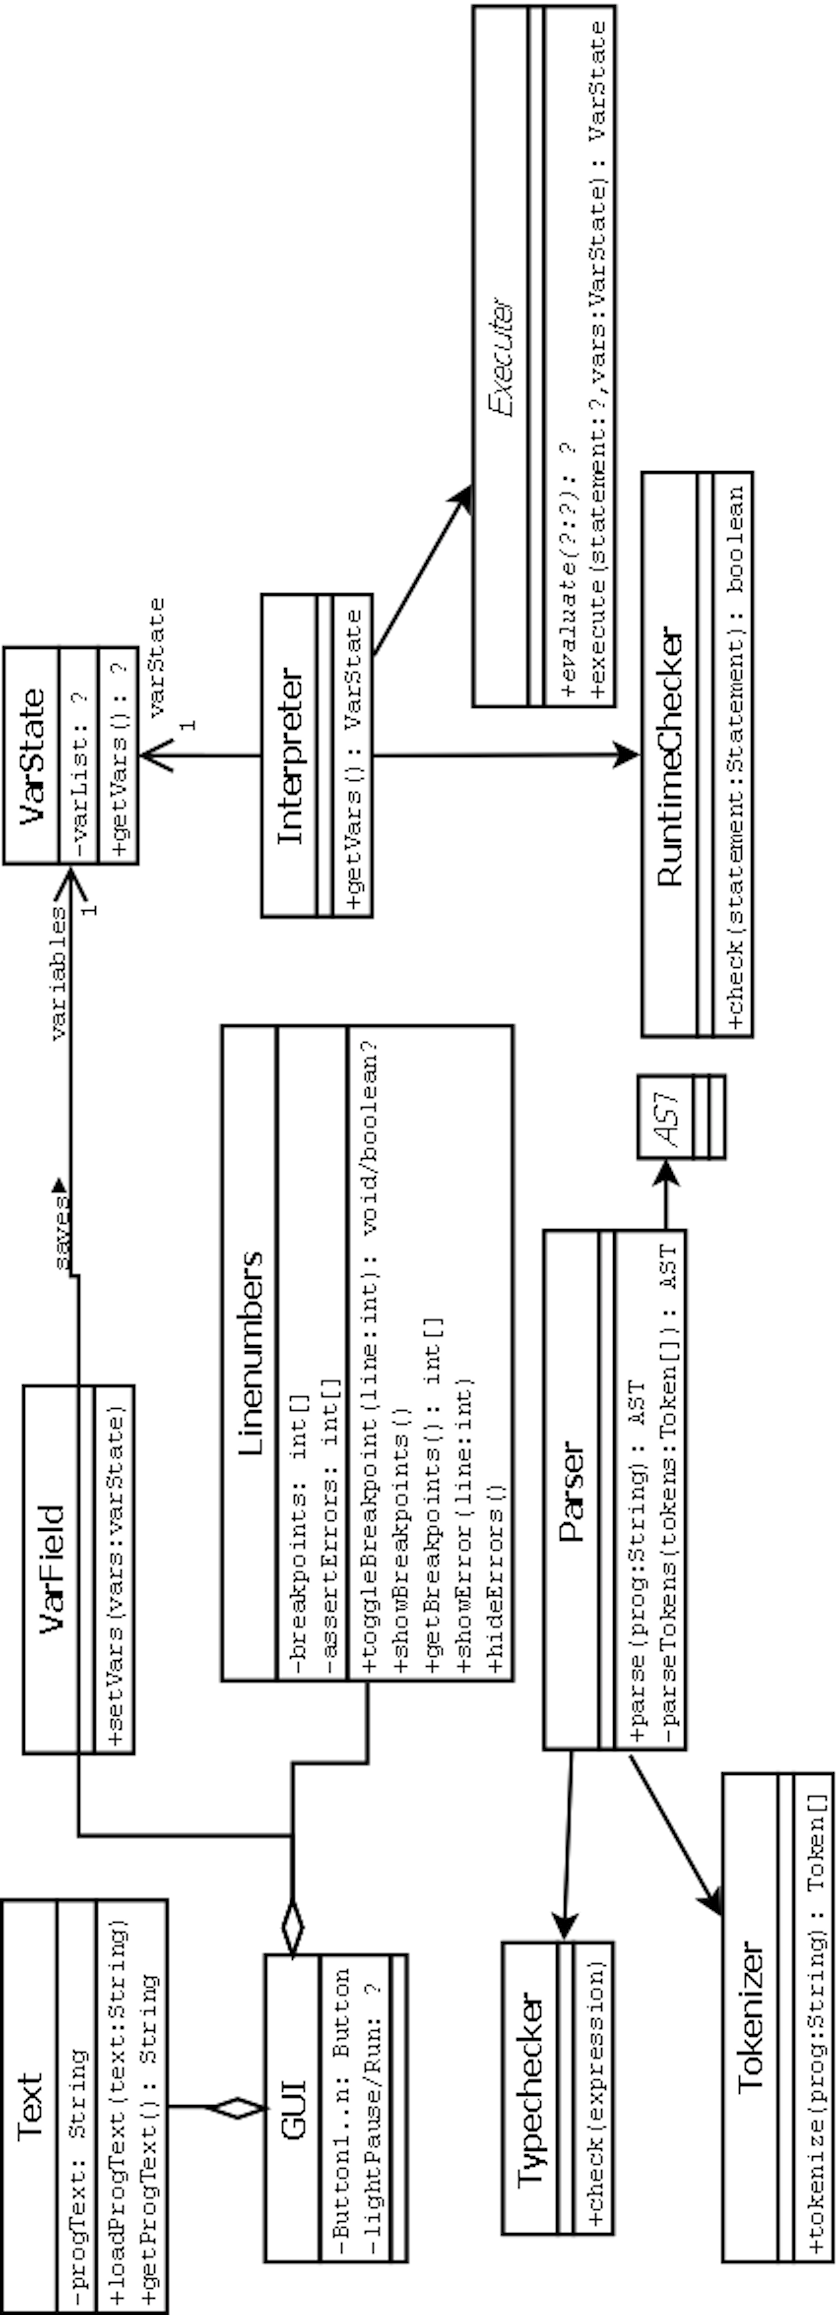
\includegraphics[scale=0.45]{ClassDiagram}
\newpage
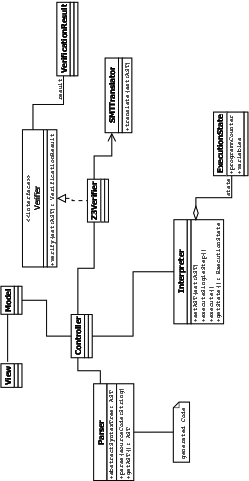
\includegraphics[scale=1.1]{ClassDiagram_alternative}
\newpage
\section{Zustandsdiagramme}
\newpage
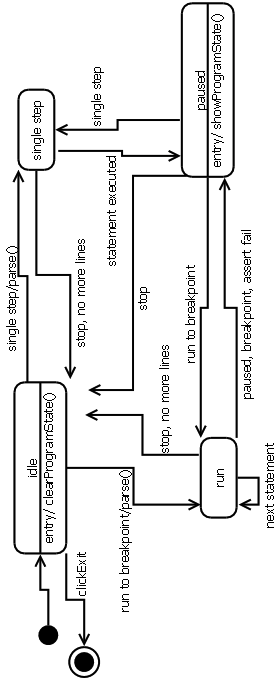
\includegraphics[scale=0.75]{Zustandsdiagramm}
\newpage
\section{Aktivtätsdiagramme}
\newpage
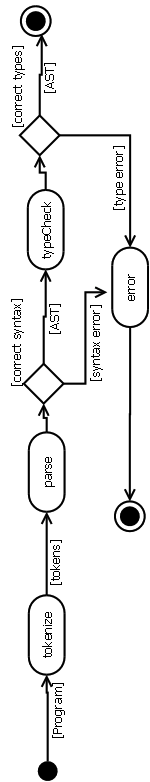
\includegraphics[scale=0.65]{Aktivitaet}
\newpage
\section{Syntax der While-Sprache}
\subsection{\"{U}bersicht der Schl\"{u}sselw\"{o}rter und Sonderzeichen}
\begin{ttfamily}
\begin{tabular}{| l  l |}
\hline
\hspace*{1cm}boolean & $\to$ type\_specifier\hspace*{2cm}\\\hline
\hspace*{1cm}else & $\to$ if\_statement\hspace*{2cm}\\\hline
\hspace*{1cm}false & $\to$ logical\_expression\\\hline
\hspace*{1cm}if & $\to$ if\_statement\\\hline
\hspace*{1cm}int & $\to$ type\_specifier\\\hline
\hspace*{1cm}return & $\to$ statement\\\hline
\hspace*{1cm}true & $\to$ logical\_expression\\\hline
\hspace*{1cm}while & $\to$ while\_statement\\\hline
\hspace*{1cm}0..9 & $\to$ integer\_literal\\\hline
\hspace*{1cm}a..z,A..Z,\_\hspace*{0.5cm} & $\to$ identifier\\\hline
\hspace*{1cm}\& & $\to$ logical\_expression\\\hline
\hspace*{1cm}| & $\to$ logical\_expression\\\hline
\hspace*{1cm}! & $\to$ logical\_expression\\\hline
\hspace*{1cm}!= & $\to$ testing\_expression\\\hline
\hspace*{1cm}== & $\to$ testing\_expression\\\hline
\hspace*{1cm}< & $\to$ testing\_expression\\\hline
\hspace*{1cm}<= & $\to$ testing\_expression\\\hline
\hspace*{1cm}> & $\to$ testing\_expression\\\hline
\hspace*{1cm}>= & $\to$ testing\_expression\\\hline
\hspace*{1cm}+ & $\to$ numeric\_expression\\\hline
\hspace*{1cm}- & $\to$ numeric\_expression\\\hline
\hspace*{1cm}* & $\to$ numeric\_expression\\\hline
\hspace*{1cm}/ & $\to$ numeric\_expression\\\hline
\hspace*{1cm}\% & $\to$ numeric\_expression\\\hline
\hspace*{1cm}, & $\to$ arglist \\
 & $\to$ parameter\_list \\
 & $\to$ variable\_declaration \\
 & $\to$ variable\_initializer\\\hline
\hspace*{1cm}; & $\to$ statement \\
 & $\to$ variable\_declaration\\\hline
\hspace*{1cm}= & $\to$ variable\_declarator\\\hline
\hspace*{1cm}( & $\to$ expression \\
 & $\to$ if\_statement \\
 & $\to$ methode\_declaration \\
 & $\to$ while\_statement\\\hline
\hspace*{1cm}) & $\to$ expression \\
 & $\to$ if\_statement \\
 & $\to$ methode\_declaration \hspace*{5cm}\\
 & $\to$ while\_statement\\\hline
\hspace*{1cm}[ & $\to$ expression \\
 & $\to$ type \\\hline
\hspace*{1cm}] & $\to$ expression \\
 & $\to$ type \\\hline
\hspace*{1cm}\{ & $\to$ statement\_block \\
 & $\to$ variable\_initializer\\\hline
\hspace*{1cm}\} & $\to$ statement\_block \\
 & $\to$ variable\_initializer\\\hline
\hspace*{1cm}\# & $\to$ comment\\\hline
\end{tabular}
\end{ttfamily}
\subsection{Startsymbol}
\texttt{compilation\_unit}
\subsection{Produktionsregeln}
\begin{verbatim}
arglist ::=  expression { "," expression }

comment ::= "#" "... text ..."

compilation_unit ::= { field_declaration }

expression ::= numeric_expression
\end{verbatim} 
		\hspace*{3cm}$\mid$ testing\_expression\\
		\hspace*{3cm}$\mid$ literal\_expression\\
		\hspace*{3cm}$\mid$ logical\_expression\\
		\hspace*{3cm}$\mid$ identifier\\
		\hspace*{3cm}$\mid$ ( "(" expression ")" )\\
		\hspace*{3cm}$\mid$ ( expression ( ( "(" $[$ arglist $]$ ")" )\\
					\hspace*{6.3cm}$\mid$ ( "[" expression "]" ) ) )
\begin{verbatim}

field_declaration ::= ( $[$ comment $]$ ( method_declaration 
\end{verbatim}
					\hspace*{7cm}$\mid$ variable\_declaration ) )
\begin{verbatim}
			
identifier ::= "a..z,A..Z,_" { "a..z,A..Z,_,0..9" }

if_statement ::= "if" "(" expression ")" statement_block [ "else" statement_block ]

integer_literal ::= ( "0..9" { "0..9" } )

literal_expression ::= integer_literal

logical_expression ::= ( "!" expression )
\end{verbatim}
		\hspace*{4.5cm}$\mid$ ( expression ( "\&" \\
				\hspace*{7.5cm}$\mid$ "|" \\
				\hspace*{7.5cm}$\mid$ ( "\&" "\&" )\\
				\hspace*{7.5cm}$\mid$ ( "|" "|" ) ) expression )\\
		\hspace*{4.5cm}$\mid$ "true"\\
		\hspace*{4.5cm}$\mid$ "false"
\begin{verbatim}
method_declaration ::= type identifier "(" [ parameter_list ] ")" ( statement_block )

numeric_expression ::= ( ( "+" 
\end{verbatim}
			\hspace*{5.3cm}$\mid$ "-" ) expression ) \\
			\hspace*{4.5cm}$\mid$ ( expression ( "+" \\
				\hspace*{7.7cm}$\mid$ "-" \\
				\hspace*{7.7cm}$\mid$ "*" \\
				\hspace*{7.7cm}$\mid$ "/" \\
				\hspace*{7.7cm}$\mid$ "\%" ) expression ) 
\begin{verbatim}					
parameter ::= type identifier

parameter_list ::= parameter { "," parameter } 

statement ::= variable_declaration
\end{verbatim}
		\hspace*{3cm}$\mid$ ( expression ";" ) \\
		\hspace*{3cm}$\mid$ ( statemen\_block )\\ 
		\hspace*{3cm}$\mid$ ( if\_statement ) \\
		\hspace*{3cm}$\mid$ ( while\_statement )\\
		\hspace*{3cm}$\mid$ ( "return" $[$ expression $]$ ";" )\\
		\hspace*{3cm}$\mid$ ( ";" ) 
\begin{verbatim}
statement_block ::= "{" { statement } "}" 

testing_expression ::= ( expression ( ">"
\end{verbatim} 
					\hspace*{7cm}$\mid$ "<" \\
					\hspace*{7cm}$\mid$ ">=" \\
					\hspace*{7cm}$\mid$ "<=" \\
					\hspace*{7cm}$\mid$ "==" \\
					\hspace*{7cm}$\mid$ "!=" ) expression ) 
\begin{verbatim}
type ::= type_specifier { "[" "]" } 

type_specifier ::= "boolean" 
\end{verbatim}
		\hspace*{3.8cm}$\mid$ "int" 
\begin{verbatim}
variable_declaration ::= type variable_declarator { "," variable_declarator } ";" 

variable_declarator ::= identifier [ "=" variable_initializer ] 

variable_initializer ::= expression
\end{verbatim}
		\hspace*{4.8cm}$\mid$ ( \{" $[$ variable\_initializer \{ "," variable\_initializer \} $]$ "\}" ) 
\begin{verbatim}
while_statement ::= "while" "(" expression ")" statement_block 
\end{verbatim}
\end{document}
